\section{Background: the inference pipeline}
\label{sec:background}

\subsection{Prefill and decode}

Let a request have prompt length \(T_p\) and generation length \(T_g\), with \(T = T_p + T_g\). Inference has two phases (Figure~\ref{fig:pipeline}):

\begin{enumerate}[leftmargin=*,itemsep=2pt]
  \item \textbf{Prefill.} The model consumes all \(T_p\) prompt tokens, writes the KV cache, and emits the first generated token. The user-visible metric is time-to-first-token (TTFT).
  \item \textbf{Decode.} The model emits tokens \(2,\ldots,T_g\) autoregressively. The user-visible metric is decode throughput (tokens/s). Each step attends over a cache of length \(T_p + t\).
\end{enumerate}

Confusing the two phases is the most common optimization error on laptops. A change that triples tokens/s can leave a 15\,s RAG pause untouched. A Flash-style kernel can collapse TTFT on long prompts while barely moving streaming speed. Product dashboards that only plot tokens/s ship demos that look fine in CI and feel broken on real prompts.

\begin{figure}[t]
  \centering
  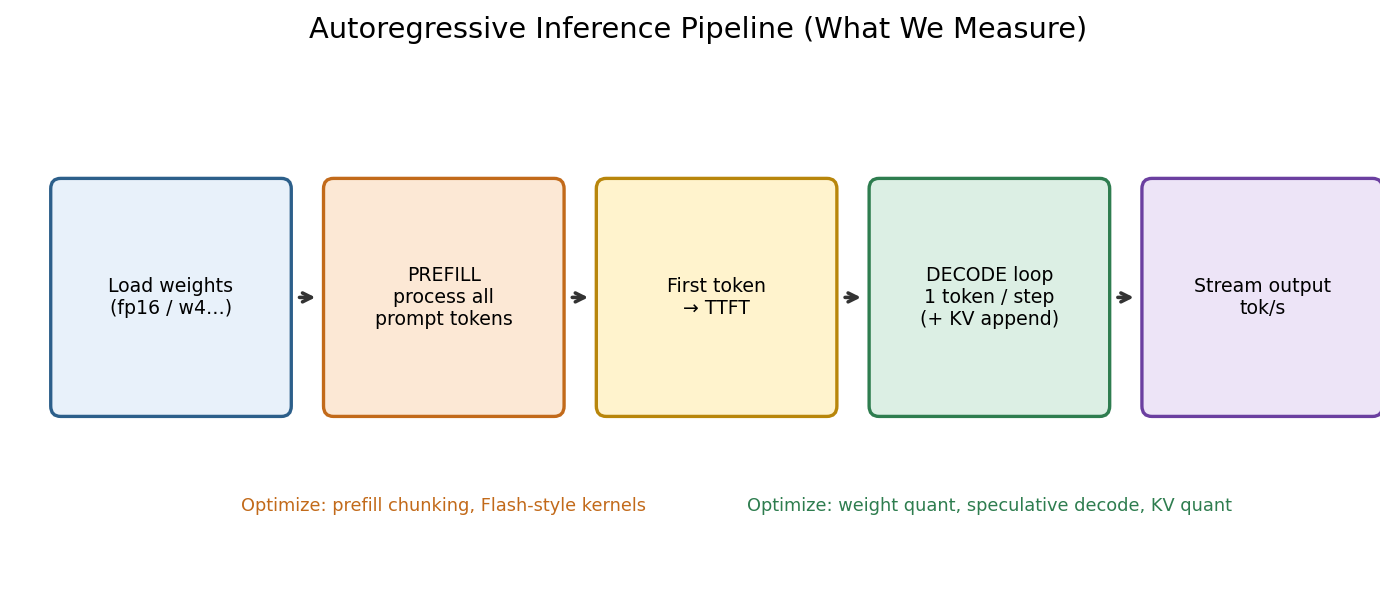
\includegraphics[width=0.98\linewidth]{figures/inference_pipeline.png}
  \caption{Single-request inference pipeline: load weights, prefill the prompt (TTFT), then autoregressive decode (tokens/s). Peak memory is a property of the whole run---the quantity everyday devices actually run out of.}
  \label{fig:pipeline}
\end{figure}

\subsection{Memory budget}

Peak resident memory is
\begin{equation}
  M_{\mathrm{peak}} \approx M_{\mathrm{weights}} + M_{\mathrm{KV}} + M_{\mathrm{act}} + M_{\mathrm{overhead}},
  \label{eq:peak}
\end{equation}
with static weights
\begin{equation}
  M_{\mathrm{weights}} \approx \frac{N \cdot b_w}{8}
  \label{eq:weights}
\end{equation}
for \(N\) parameters at \(b_w\) bits, and a KV cache
\begin{equation}
  M_{\mathrm{KV}} \approx 2\, L\, H_{\mathrm{kv}}\, T\, D\, \frac{b_{\mathrm{kv}}}{8}
  \label{eq:kv}
\end{equation}
for \(L\) layers, \(H_{\mathrm{kv}}\) key/value heads, head dimension \(D\), sequence length \(T\), and \(b_{\mathrm{kv}}\) bits per cached element~\citep{pope2022efficiently,ainslie2023gqa}. The factor of two is the pair \((K,V)\). Grouped-query and multi-query attention reduce \(H_{\mathrm{kv}}\) relative to query heads~\citep{shazeer2019mqa,ainslie2023gqa}. \(M_{\mathrm{overhead}}\) includes the framework, allocator fragmentation, and---critically on everyday devices---whatever the OS and apps already hold.

For a Llama-class 8B model, \(b_w = 16\) costs \(\approx 16\)\,GB of weights. At \(b_w = 4\) the same term is \(\approx 4\)\,GB. For \(L=32\), \(H_{\mathrm{kv}}=8\), \(D=128\), \(T=640\), FP16 KV is \(\approx 84\)\,MB; 4-bit KV is \(\approx 21\)\,MB. At \(T=4096\), FP16 KV is \(\approx 536\)\,MB. Weights set the \emph{floor}; KV sets the \emph{slope} in \(T\). Short-chat benches are weight-dominated and will lie about KV optimizations (Section~\ref{sec:kv}).

\subsection{Roofline view of decode}

When a decode step is memory-bandwidth bound~\citep{williams2009roofline},
\begin{equation}
  \mathrm{tok/s} \approx \frac{B_{\mathrm{mem}}}{B_{\mathrm{token}}},
  \label{eq:roofline}
\end{equation}
where \(B_{\mathrm{mem}}\) is sustained DRAM (or HBM) bandwidth and \(B_{\mathrm{token}}\) is bytes moved per generated token---dominated by reading the weights. Reducing \(b_w\) therefore raises tokens/s \emph{and} lowers \(M_{\mathrm{weights}}\). On a laptop this is why 4-bit is not only a fit trick: Llama~3.1~8B on an M3 moves from 5.8 to 20.5 tokens/s when \(b_w: 16 \to 4\), close to the byte-ratio prediction after kernel overheads.

Prefill can be much more compute- or attention-IO-bound as \(T_p\) grows. The same 4-bit checkpoint that streams well can still post a 15\,s TTFT at \(T_p=2048\).

\subsection{Unified memory versus discrete GPUs}

On a discrete GPU, weights live in HBM; the host CPU has a separate DRAM pool; PCIe is an explicit copy path. On Apple Silicon, CPU, GPU, and Neural Engine share one unified DRAM pool~\citep{apple2020silicon,mlx2023} (Figure~\ref{fig:um}). There is no host--device copy in the CUDA sense, and also \emph{no private VRAM ceiling}. Local 8B inference on a 24\,GB Mac is a packing problem first and a kernel problem second.

\begin{figure}[t]
  \centering
  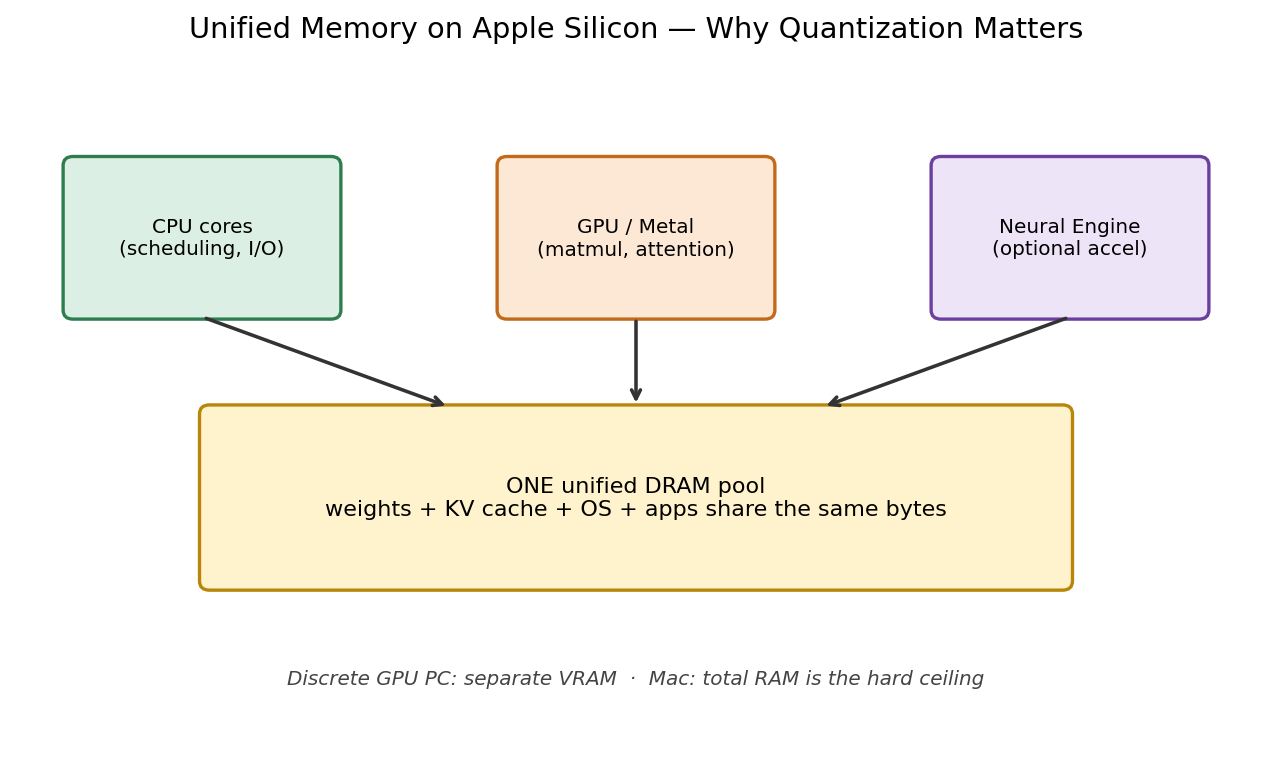
\includegraphics[width=0.92\linewidth]{figures/unified_memory.png}
  \caption{Unified memory on Apple Silicon: weights, KV cache, activations, and the operating system share one DRAM pool. Capacity planning \emph{is} the first optimization on everyday devices.}
  \label{fig:um}
\end{figure}

\subsection{Quality as a constraint, not a metric to maximize in this paper}

We do not claim that 4-bit matches FP16 on every reasoning bench. GPTQ/AWQ-class 4-bit is widely treated as the practical default for local chat and coding~\citep{frantar2022gptq,lin2023awq}; 2-bit and naive 3-bit remain research-to-product. A responsible local stack uses 4-bit as the daily driver and keeps a W8/FP16 checkpoint for eval nights (Section~\ref{sec:decision}).
